\documentclass{VUMIFPSkursinis}
\usepackage{algorithmicx}
\usepackage{algorithm}
\usepackage{algpseudocode}
\usepackage{amsfonts}
\usepackage{float}
\usepackage{amsmath}
\usepackage{bm}
\usepackage{caption}
\usepackage{color}
\usepackage{float}
\usepackage{graphicx}
\usepackage{listings}
\usepackage{subfig}
\usepackage{ltablex}
\usepackage{longtable}
\usepackage{wrapfig}
\usepackage{subfig}
\usepackage{pbox}
\renewcommand{\labelenumii}{\theenumii}
\renewcommand{\theenumii}{\theenumi.\arabic{enumii}.}
\renewcommand{\labelenumiii}{\theenumiii}
\renewcommand{\theenumiii}{\theenumii\arabic{enumiii}.}
% Titulinio aprašas
\university{Vilniaus universitetas}
\faculty{Matematikos ir informatikos fakultetas}
\department{Programų sistemų katedra}
\papertype{Projektinis darbas}
\title{Internetinio banko tinklalapis}
\titleineng{Bankininkystė}
\status{3 kurso 3 grupės studentai}
\author{Justas Tvarijonas}
\secondauthor{Džiugas Mažulis}   
\thirdauthor{Michal Stankiewicz}   
\supervisor{Kristina Lapin, Doc., Dr.}
\date{Vilnius – \the\year}

\begin{document}
\maketitle
\sectionnonum{Anotacija}
\subsectionnonum{Darbo tikslas}
Naudojant į vartotoją orientuotą dizainą palengvinti bei pagerinti Swedbank internetinio banko puslapio naudojamumą bei efektyvumą taip padidinant puslapio našumą bei vartotojų pasitenkinimą.
\subsectionnonum{Darbo pasiskirstymas}
\begin{itemize}
	\item Justas Tvarijonas - tvarijonasjustas@gmail.com \newline
	Įvadas, kompiuterizuojamų veiklų analizė, įkvepiantys interfeisai.
	\item Džiugas Mažulis - džiugas.mažulis@gmail.com \newline 
	Kompiuterizuojamų veiklų analizė, įkvepiantys interfeisai.
	\item Michal Stankevič - michal.stankevic@gmail.com \newline
	 Kompiuterizuojamų veiklų analizė, įkvepiantys interfeisai.
\end{itemize}
\tableofcontents
\sectionnonum{Įvadas}
\subsectionnonum{Dalykinė sritis}
Internetinė bankininkystė.
\subsectionnonum{Probleminė sritis}
Vartotojų patogumo gerinimas, patogus informacijos pateikimas. Sistemos pateikimas aiškenia vartotojo sąsaja.
\subsectionnonum{Naudotojai}
	Banko klientas - turi galimybę atlikti mokėjimus, peržiūrėti sąskaitos išrašus, kurti mokėjimo ruošinius, ieškoti reikalingos informacijos.
\subsectionnonum{Darbo pagrindas}
Pirmojo laboratorinio darbo reikalavimai.
\section{Būsimos sistemos įtakojamų asmenų kategorijos}
\subsection{Suinteresuotų asmenų grupės}
\begin{itemize}
	\item Pirminiai - Banko klientai, betarpiškai naudojasi sistema.
	\item Antriniai - neegzistuoja.
	\item Tretiniai - Kiti bankai, kurių klientų skaičių įtakoja šio banko sekmė, bei akcininkai, kurių pajamos priklauso nuo banko sekmės.
\end{itemize}
\section{Banko klientų poreikiai}
\subsection{Naudotojų charakteristikos}
\subsubsection{Informacinių technologijų priemonės}
\begin{itemize}
	\item Išmanusis telefonas (naršyklė bei smard-id).
	\item Mobilusis parašas.
	\item Asmeninių kompiuterių naršyklės.
	\item Planšetinių kompiuterių naršyklės.
\end{itemize}
\subsubsection{Motyvacija ir galimybės tobulinti įgūdžius}
\begin{itemize}
	\item Klientai turi skirtingus IT įgūdžius.
	\item Klientai skirtingais dažnumais naudojasi elektronine bankininkyste.
\end{itemize}
\subsubsection{Veiklų kontekstai}
\begin{itemize}
	\item Veikla yra pertraukiama. Klientas gali suformuluoti mokėjimą, tada užsiimti kita veikla ir vėliau grįžti užbaigti mokėjimą.
	\item Mokėjimai atliekami su dideliu susikaupimu.
	\item Naudojimasis sistema atliekamas saugioje aplinkoje.
	\item Paprastai sistema naudojama turint aiškų tikslą.
	\item Apsilankymas banko svetainėje paprastai trunka iki 30 minučių.
	\item Banko klientai svetainėje apsilanko bent kelis kartus į mėnesį.
\end{itemize}
\subsubsection{Naudotojų tipas}
\begin{itemize}
	\item Naujokai - šie naudotojai iš anksto nežino kur jiems reikia spausti norint pasiekti norimą tikslą. Juos gąsdina sudėtingas ir pilnas funkcionalumo pagrindinis langas, tačiau pastebi didesniu mygtukus ar užrašus, kurie skelbia jiem naudingą informaciją.
	\item Vidutiniškai patyrę - šie naudotojai banko paslaugomis naudojasi pakankamai dažnai, kad efektyviai atliktu įprastus veiksmus, tačiau susiduria su problemomis norėdami atlikti sudėtingesnias operacijas.
	\item Ekspertai - šie sistemos naudotojai puikiai išmano sistemą, jiems patogus didelio funkcionalumo sudėtingas interfeisas. Juos erzina didelis žingsnių skaičius bei į naujokus orientuota vartotojo sąsaja.
\end{itemize}
\subsection{Kompiuterizuojamų veiklų analizė}
\subsubsectionnonum{Mokėjimo pavedimų koncepcinis scenarijus}
Kęstas nori pervesti pinigus į draugo sąskaitą, tačiau pagrindiniame lange neranda pinigų pavedimo funkcijos. Nežinodamas ar „Vietiniai mokėjimai“ yra tai, ko jam reikia, jis meniu juostoje paspaudžia „Mano bankas“. Neradęs tinkamo pasirinkimo Petras meniu juostoje spusteli „Kasdieninės paslaugos“, tačiau jį suglumina skiltyje „Mokėjimai“ atsiradę pasirinkimai: „Mokėjimo pavedimai“, „Vietiniai mokėjimai“, „Įmokos“, „E. sąskaitos“. Pasirinktame „Mokėjimo pavedimai“ lange klientas nežino ką įvesti „Gavėjo pavadinimas“ skiltyje, tik paspaudęs ant klaustuko simbolio sužino, jog įvesti reikia draugo vardą ir pavardę. Visą sąskaitos numerį Petras turi vesti ranka, nors jau yra ankščiau pervedęs draugui pinigų. Įvedęs visus duomenis bei paspaudęs toliau vartotojas atsiduria vietinių mokėjimų lange, kuriame turi įvesti gavėjo šalį, adresą. Paspaudęs mygtuką „Toliau“ Petras perveda draugui pinigus.
\subsubsectionnonum{Mokėjimo pavedimų veiklų charakteristikos}
Veiklos dažnis: mokėjimo pavedimai yra esminė bei dažniausiai naudojama elektroninės bankininkystės funkcija: apie 10-15 kartų per mėnesį. Privaloma užtikrinti akivaizdų, vienprasmišką bei vieno mygtuko paspaudimu pasiekiamą pagrindinį funkcionalumą norint greitai ir rezultatyviai atlikti pavedimus. Įvesties langai turi būti aiškiai suprantami bei pasirinkus siųsti pinigus sistema privalo pasiūlyti pasirinkti gavėją iš gavėjų sąrašo arba ankstesnių gavėjų. Iš banko sąskaitos galima atpažinti gavėjo šalį, todėl sistema neturėtų reikalauti šio parametro. \par 
Veiklos trukmė: mokėjimo pavedimas internetinės bankininkystės sistemoje užtrunka nuo 2 iki 5 minučių.
\subsubsectionnonum{Mokėjimo pavedimų problemos ir tobulinimo galimybės}
\begin{itemize}
	\item Mokėjimo pavedimo funkcija vizualiai neatkreipia dėmesio bei yra neaiškaus pavadinimo.
	\item Mokėjimų skiltyje per daug pavedimo interpretacijų.
	\item Įvesties lauko „Gavėjo pavadinimas“ pavadinimas neaiškiai apibrėžia reikalaujamus duomenis.
	\item Sistema neteikia galimybės pasirinkti anksčiau naudotą gavėją arba gavėją iš sąrašo.
	\item Sistema iš banko sąskaitos neatpažįsta gavėjo šalies.
\end{itemize}
\subsubsectionnonum{Būsimasis patobulintas scenarijus}
\begin{center}
\textbf{Vartotojas norėdamas atlikti mokėjimo pavedimą:}
\end{center}
\begin{enumerate}
	\item Pagrindiniame lange į teksto lauką įveda pinigų sumą bei paspaudžia mygtuką „Siųsti pinigus“
	\item Įvesdamas duomenis
	\begin{enumerate}
		\item Pasirenka gavėją iš „Gavėjų sąrašo“
		\item Pasirenka gavėją iš „Ankstesni“
		\item Suveda gavėjo sąskaitos numerį
		\begin{enumerate}
			\item Į lauką „Gavėjo vardas, pavardė (įmonės pav.)“ įveda gavėjo pavadinimą
		\end{enumerate}
	\end{enumerate}
	\item Paspaudžia mygtuką „Patvirtinti mokėjimą“
\end{enumerate}
\subsubsectionnonum{Informacijos paieškos koncepcinis scenarijus}
Jonas ieško kaip gali išsinuomuoti saugyklą banke, pasirinkęs "Mano bankas" pamato ilgą sarašą informacijos, tačiau jį peržvelgęs nerando norimos informacijos, dar kartą atydžiai peržvelgia naudingos informacijos nuorodų grupę, tačiau vistiek neranda norimo puslapio nuorodos. Tik tada pamato, kad dešiniąjame lango kampe yra paieškos logotipas, jį paspaudus įveda "seifo nuoma" į paieškos langą, tačiau paieška neranda nieko prasmingo. Galiausiai neapsikentęs jis parašo žinutę banko dorbuotojui, kuris jam atsiunčia nuorodą į ieškomą puslapį, bei praneša, kad šios informacijos reikia ieškoti neprisijungus prie banko. 
\subsubsectionnonum{Informacijos paieškos veiklų charakteristikos}
Veiklos dažnis: Informacijos paieška banko internetinėje svetainėje paprastai nėra dažna: apie 5-6 kartus į metus, todėl jos pasiekimas turėtų būti pakankamai akivaizdus. Neradus rezultatų siūlytų panašius arba atidaryti bendravymo gyvai langą, kuriame vartotojas galėtų sužinoti norimą informaciją. \par
Veiklos trukmė: Informacijos paieška vidutiniškai užtrunka neilgai - iki 5 minučių.
\subsubsectionnonum{Informacijos paieškos problemos ir tobulinimo galimybės}
\begin{itemize}
	\item Paieškos lango pozicija nėra akivaizdi.
	\item Paieškos rezultatų negalima sugrupuoti.
	\item Paieška informacijos ieško ne iš viso galimo informacinio lauko.
	\item Neradus rezultatų nėra pasiūlomas joks situacijos sprendimas.
\end{itemize}
\subsubsectionnonum{Būsimasis patobulintas scenarijus}
\begin{center}
	\textbf{Vartotojas norėdamas surasti informacijos apie seifų nuoma:}
\end{center}
\begin{enumerate}
	\item Vartotojas paspaudžia ant paieškos mygtuko pagrindiniame lange
	\item Sistema atidaro naują langą, kuriame vartotojas gali įvesti raktinius žodžius
	\item Vartotojas įvedęs raktinius žodžius gali atidaryti vieną iš rastų rezultatų, filtruoti rezultatus pagal kategorijas, pažiūrėti alternatyvius siūlomus raktinius žodžius.
	\begin{enumerate}
		\item atidarius vieną iš rezultatų:
		\begin{enumerate}
			\item tame pačiame lange atidaromas pasirinkto rezultato puslapis
			\item vartotojas vienu paspaudimu gali grįžti atgal į rezultatų sąrašą
		\end{enumerate}
	\end{enumerate}
	\begin{enumerate}
		\item pasirinkęs filtravimą pagal kategoriją: vartotojas mato tik tuos rezultatus, kurie priklauso pasirinktai kategorijai.
		\begin{enumerate}
			\item vartotojas mato tik tuos rezultatus, kurie priklauso pasirinktai kategorijai
			\item vartotojas bet gali atšaukti filtravimą
		\end{enumerate}
	\end{enumerate}
	\begin{enumerate}
		\item pasirinkęs peržiūrėti alternatyvius siūlomus variantus:
		\begin{enumerate}
			\item gali pasirinkti vieną iš siūlomų variantų ir ieškoti iš naujo
			\item toliau žiūrėti jau rastus rezultatus
		\end{enumerate}
	\end{enumerate}
\end{enumerate}
\subsubsectionnonum{Mokėjimo ruošinio sukūrimo koncepcinis scenarijus}
Antanas nori sukurti mokėjimo ruošinį pagal seniau atliktą mokėjimą, tačiau, kadangi nežino, kaip tai atlikti atlikti jis bando orientuotis pagal pavadinimus. Pasirinkęs kasdienes paslaugas ir peržvelges visus variantus per kelias minutes randa pasirinkimą "Mokėjimo ruošiniai" bei ant jo paspaudžia. Atsidariusiame lange pasirenka "Sukurti vietinį mokėjimo ruošinį", tačiau atsidarius naujam langui pamato, kad nebus pasirinkimo sukurti ruošinį pagal buvusį mokėjimą, todėl, norėdamas sužinoti gavėjo duomenis, nueina peržvelgti buvusius mokėjimus. Ten susiradęs reikiamą mokėjimą pamato, kad gali sukurti ruošinį pagal šį mokėjimą, taip ir padaro.
\subsubsectionnonum{Mokėjimo ruošinio sukūrimo veiklų charakteristikos}
Veiklos dažnis: Mokėjimo ruošinio sukūrimas yra retas veiksmas, todėl vartotojas kiekvieną kartą jį atlieka kaip iš naujo, todėl jis turėtų būti pakankamai aiškus ir paprastas. \par
Veiklos trukmė: Mokėjimo ruošinio sukūrimas turėtų užtrukti iki 10 minučių.
\subsubsectionnonum{Mokėjimo ruošinio sukūrimo problemos ir tobulinimo galimybės}
\begin{itemize}
	\item Mokėjimo ruošinių lange nėra pasirinkimo sukurti ruošinį pagal buvusius mokėjimus
	\item Mokėjimo ruošinių paieška galima tik pagal jo pavadinima (tačiau ne pagal gavėją bei mokėjimo paskirtį)
\end{itemize}
\subsubsectionnonum{būsimasis patobulintas scenarijus}
\begin{center}
	\textbf{Vartotojas norėdamas sukurti mokėjimo ruošinį:}
\end{center}
\begin{enumerate}
	\item Vartotojas atsidaro mokėjimo ruošinių langą bei pasirenka sukurti vietinį mokėjimo ruošinį.
	\item Sistema vartotojui duoda pasirinkima kurti mokėjimo ruošinį pagal buvusį mokėjimą arba kurti be jo.
	\begin{enumerate}
		\item Vartotojui pasirinkus kurti ruošinį pagal buvusį mokėjimą:
		\begin{enumerate}
			\item Sistema vartotojui atidaro naują langą, kuria rodomi buvę Mokėjimai
			\item Vartotojas susirandą norimą mokėjimą bei jį pasirenka
			\item Sistema vartotoja nukelia į mokėjimo ruošinio sukurimo langą, kuriame automatiškai užpildo laukus pagal pasirinktą buvusį mokėjimą
			\item Vartotojas, sutikrines mokėjimo ruošinio laukus, pasirenka jį išsaugoti
		\end{enumerate}
		\item Vartotojui pasirinkus kurti mokėjimo ruošinį nuo nulio:
		\begin{enumerate}
			\item Sistema vartotojui atidaro mokėjimo ruošinio sukūrimo langą, kuriame visi laukai yra tušti
			\item Vartotojas suveda reikiamus duomenis bei išsaugo mokėjimo ruošinį
		\end{enumerate}
	\end{enumerate}
\end{enumerate}
\subsection{Panaudojamumo siekiai ir matai}
\begin{itemize}
	\item Naudotojas galės filtruoti paieškos rezultatus pagal skirtingas rastas grupes
	\item Naujas vartotojas paieškos langą surasti galės ne per ilgesnį laiką, nei 30 sekundžių.
	\item 90\% paieškų bus rezultatyvios.
	\item Vartotojui įvedus ne mažiau, kaip 3 simbolius į paieškos langą bus siūlomi pilni paieškos tekstai
	\item Vartotojas galės mokėjimo ruošinių ieškoti pagal pavadinimą, gavėją bei mokėjimo paskirtį
	\item Mokėjimo ruošinio sukurimo langą vartotojas galės pasiekti ne per daugiau, negu 3 mygtukų paspaudimus.
	\item Kurdamas mokėjimo ruošinį vartotojas gaus bent 2 pasirinkimus jam sukurti.
	\item Klientas galės įvesti sumą bei pradėti pavedimą pagrindiniame lange.
	\item Klientas galės pasirinkti gavėją iš gavėjų arba ankstesnių gavėjų sąrašų.
	\item Rinkdamasis gavėją iš pateiktų sąrašų, klientas galės atlikti pavedimą 3 mygtukų paspaudimu.
	\item Pavedimo atlikimas truks ne ilgiau kaip 2 minutes.
	\item 95\% klientų iš pirmo karto ras kaip atlikti pavedimą.
\end{itemize}
\pagebreak
\section{Įkvepiančios esamų interfeisų idėjos}
\begin{figure}[!htb]
	\begin{center}
	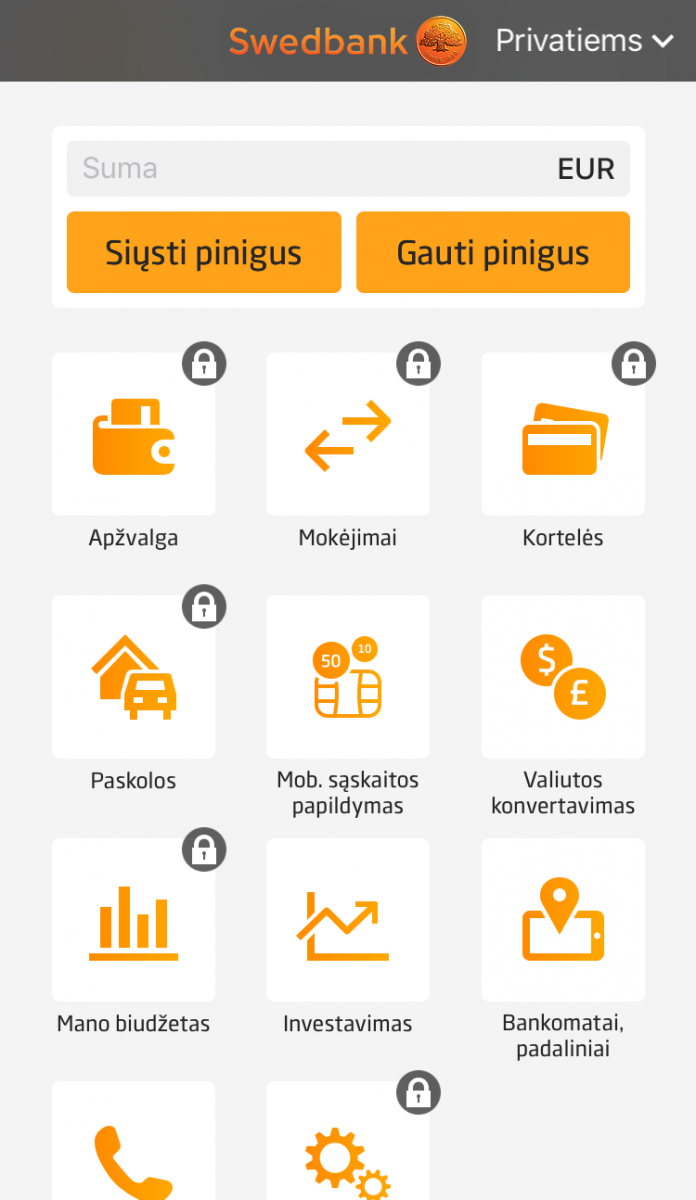
\includegraphics[scale=0.4]{mobileApp.png}
	\end{center}
  \caption{Mygtukai iš mobiliosios aplikacijos}
	\label{fig:mobileApp}
	Nauda: Piktogramos visiems labiau suprantamos, lengviau skaitomos, jų pagalba norimus puslapius galima rasti greičiau.
\end{figure}
\begin{figure}[!htb]
	\begin{center}
	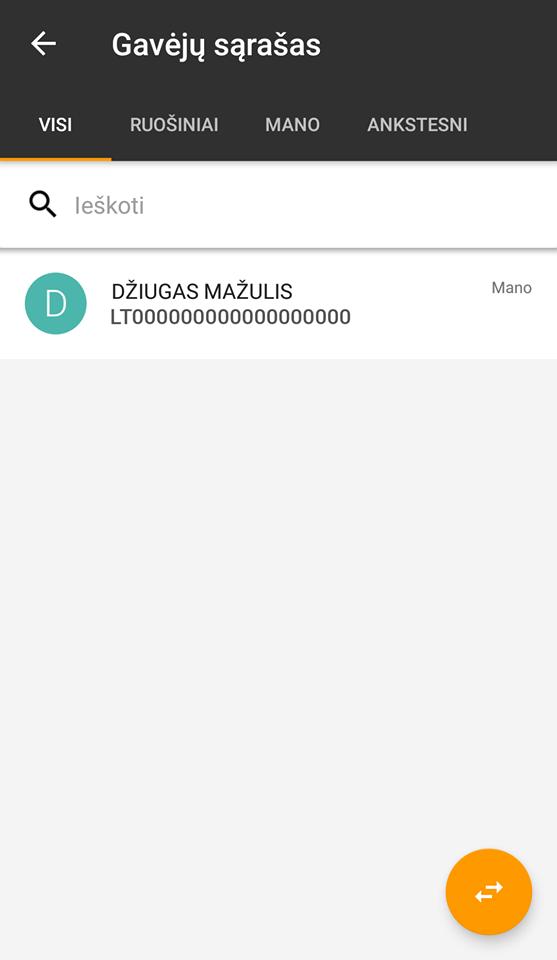
\includegraphics[scale=0.4]{mobileAppRecipientList.png}
	\end{center}
  \caption{Gavėjų sąrašas aplikacijoje}
	\label{fig:mobileAppRecipientList}
	Nauda: galima pasirinkti gavėją bei visą būtiną informaciją iš gavėjų sąrašo.
\end{figure}
\begin{figure}[!htb]
	\begin{center}
	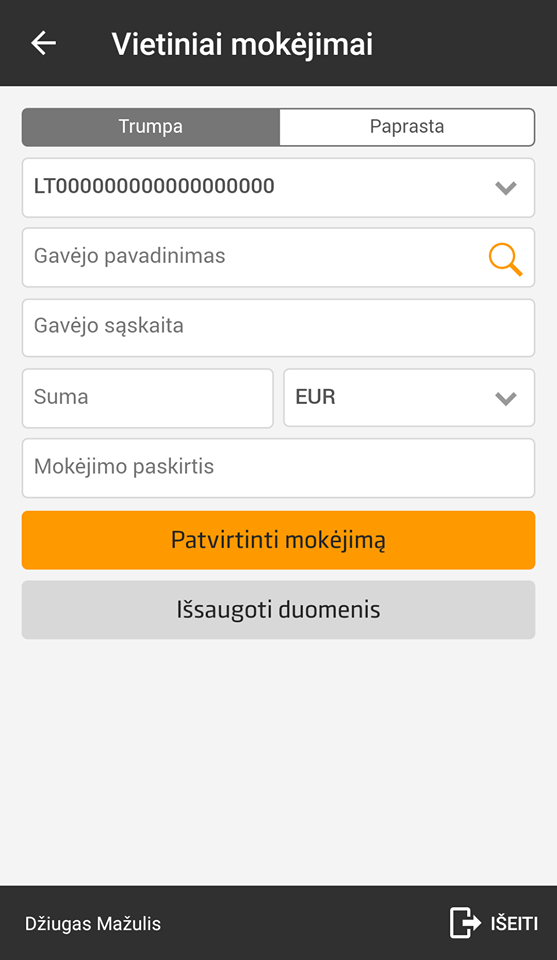
\includegraphics[scale=0.4]{mobileAppPaymentForm.png}
	\end{center}
  \caption{Mokėjimo forma aplikacijoje}
	\label{fig:mobileAppPaymentForm}
	Nauda:  įvesti reikia tik būtiną, esminę informaciją, vartotojo neprašo įvesti nebūtinos informacijos.
\end{figure}
\begin{figure}[!htb]
  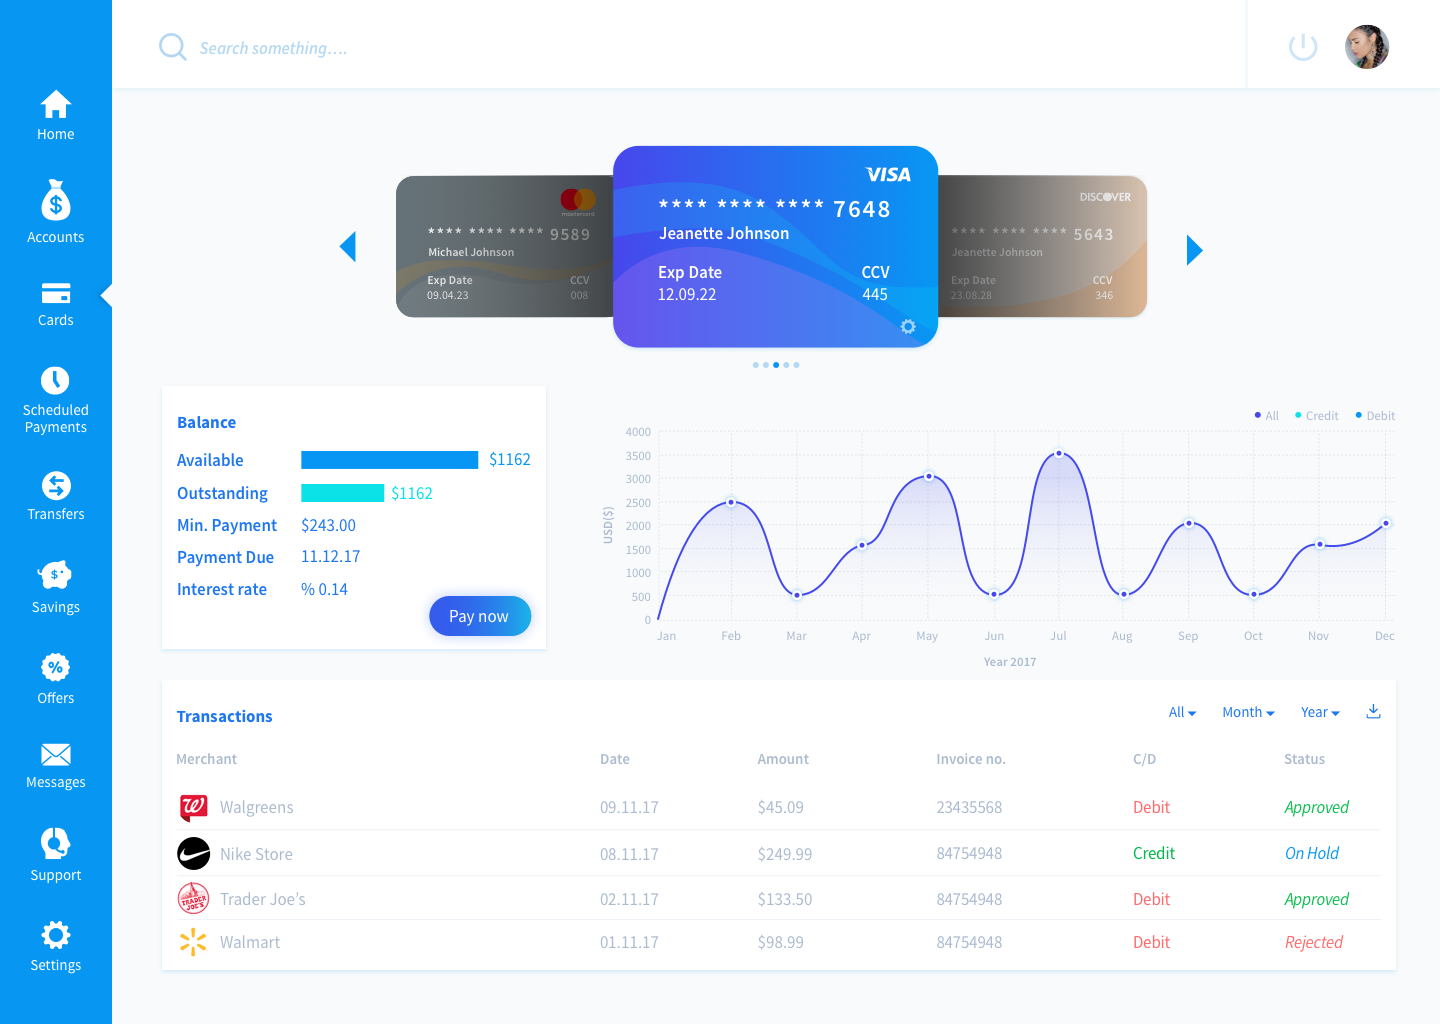
\includegraphics[width=\linewidth]{iconPlacement.png}
  \caption{Mygtukų išdėstymas svetainėje}
	\label{fig:iconPlacement}
	Nauda: Vartotojui aiškus meniu, greitas vaikščiojimas tarp puslapių.
\end{figure}
\begin{figure}[!htb]
  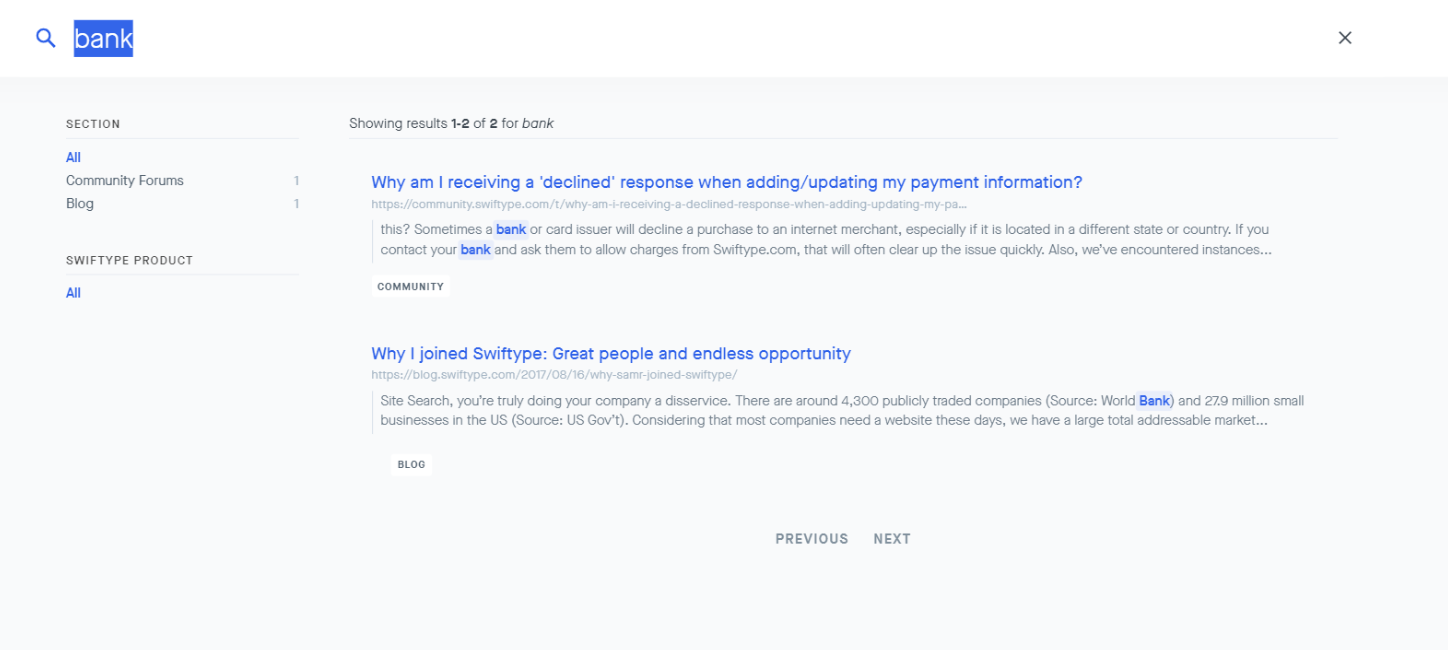
\includegraphics[width=\linewidth]{SearchWindow.png}
  \caption{Informacijos paieškos langas}
	\label{fig:searchWindow}
	Nauda: Vendant tekstą ieškoma po kiekvieno įvesto simbolio, galima filtruoti pagal skirtingas grupes.
\end{figure}
\begin{figure}[!htb]
	\begin{center}
	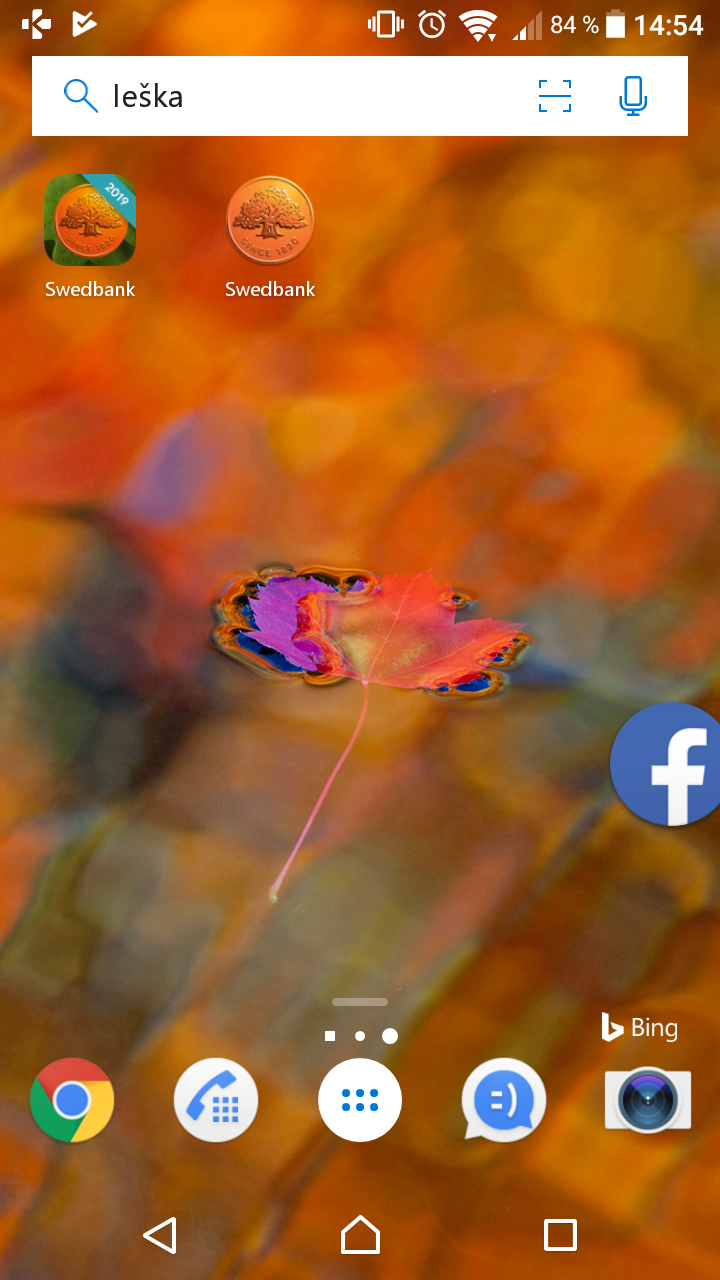
\includegraphics[scale=0.2]{pagalbaGyvai.png}
	\end{center}
  \caption{Piktograma susisiekimui su pagalba gyvai}
	\label{fig:pagalbaGyvai}
	Nauda: greitas pagalbos naudojantis puslapiu pasiekimas, piktogramą galima nesunkiai patraukti.
\end{figure}
\end{document}
